% CUSTOM TEMPLATE FOR SOLUTIONS STARTS
\documentclass[answers]{exam}
 
 \usepackage{graphicx}
 \usepackage{float}
 \usepackage{amsmath}
 \usepackage{amsfonts}
 \usepackage{framed}
 \usepackage{algorithmicx}
 \usepackage{algpseudocode}
 \newcommand{\ans}[1]{\begin{framed}{\textbf{Answer:} #1}\end{framed}}
 \newcommand{\sol}{\uplevel{\textsc{Solution:}}}
 \newenvironment{answer}{%
     \renewcommand{\solutiontitle}{\noindent\textbf{Answer:}\enspace}
     \begin{solution}
     }{%
     \end{solution}
     \renewcommand{\solutiontitle}{\noindent\textbf{Solution:}\enspace}
 }
% CUSTOM TEMPLATE FOR SOLUTIONS ENDS

% First we setup the header and footer
\pagestyle{headandfoot}
\runningheadrule
\runningfootrule
\header{COL351: Analysis and Design of Algorithms (CSE, IITD, Semester-I-2020-21)}{}{Major Exam}
\footer{}{\thepage  \, of \numpages}{}
 
% We want the points for each question displayed on the left
%\pointname{points}
%\pointsinmargin
 
% Automatically total the points - make sure to compile TWICE
\addpoints

\begin{document}


\vspace{0.1in}


\vspace{0.1in}
% Some general text together with number of questions and total points possible
There are \numquestions\, questions for a total of \numpoints\, points.
\vspace{0.1in}
\hrule
 \vspace{0.2in}
\begin{questions}
 
\question[5] 

Recall the domino tiling problem of Quiz-5 given below:

    There is an $n \times n$ grid in which some cells are empty and some are filled. The empty/filled cells are given by an $n \times n$, 0/1 matrix $F$. Cell $(i, j)$ is empty iff $F[i, j] = 0$. You
    have unbounded supply of $2 \times 1$ tiles (called dominoes). Each domino could be placed on the empty cells of the grid in horizontal and vertical manner (note that you need two consecutive
    empty cells on the grid for doing this). The problem is to determine if the grid can be covered by placing these $2 \times 1$ dominos such that each empty cell is covered by exactly one domino. 

Consider the following algorithm for this problem:

    \begin{center}
        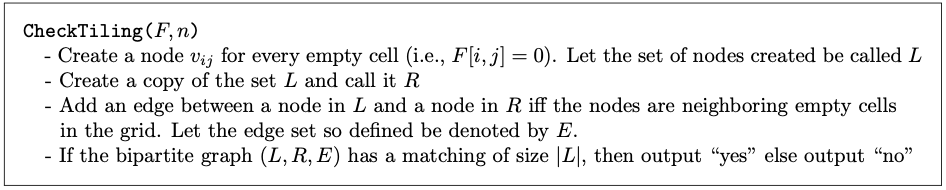
\includegraphics{major/Tiling-algo.png}
    \end{center}

Prove or disprove the following statement:

    The above algorithm is correct.

[Since this is a proof question, there will be emphasis on clarity.]

    \begin{solution}

        \textbf{Answer:} Yes, the algorithm is correct

        \textbf{Proof:}

Call this graph $G$. Call any given valid covering of the board by dominos a \textit{tiling}.

        \textbf{Claim 0:} This graph is bipartite.
        
        \textit{Proof:} This is true by construction, since we don't add edges between vertices in the same set.

        \textbf{Claim 1:} There is a perfect matching in this graph $\implies$ there is a tiling.

        \textit{Proof:} We break into two claims.

        \textbf{Claim 1.1:} If there is a perfect matching in this graph, then there is a perfect matching where $(u, v)$ is in the matching implies that $(v, u)$ in the matching.

        \textit{Proof:} Consider the sets $S, T$ in the graph where $S$ corresponds to the empty cells with odd sum of coordinates and $T$ for the remaining empty cells. Note that the graph has no
        edges between $S$ and $S$ on the left and right sides respectively, and similarly for $T$ (this is because any two adjacent cells have opposite parities of the sum of coordinates). Since there
        is a perfect matching, we have all vertices of $S$ on the left matched with all vertices of $T$ on the right. Call the subgraph induced by this $G'$. Then copy $S$ and $T$ and all the edges
        between them, and put the copy of $S$ in the right side and the copy of $T$ in the left side of $G'$ (not $G$). Note that this graph has the same set of vertices as the original graph, and it also has a perfect matching, and we are done.

        \textbf{Claim 1.2:} Claim 1 is true.

        \textit{Proof:} Suppose a perfect matching exists. Consider a perfect matching. Using the previous lemma, construct another perfect matching. Hence for each edge $(u, v)$ in the graph, since
        $(u, v)$ is an edge in $G$, $u$ and $v$ must be adjacent cells of the grid which are both unfilled. Hence, we can place a domino covering these two tiles. Now to show that this tiling is valid, note that if there were two dominos intersecting at a cell, then in the perfect matching, we must have had two edges sharing an endpoint, which is impossible due to it being a valid matching. To show that it covers all the unfilled cells, note that since the perfect matching matches all the vertices of the bipartite graph (i.e., for each vertex, there is an edge whose endpoint it is), for each unfilled cell, we must have a domino covering it. Hence we have shown that for a perfect matching in the graph, there is a tiling.

        \textbf{Claim 2:} There is a tiling $\implies$ there is a perfect matching in this graph.

        For any domino, note that it covers two adjacent squares. Add the edges $(u, v)$ and $(v, u)$ between these two cells into a set $X$ (and do this for all dominos). Note that since no two
        dominos overlap, no two edges share a vertex, and thus these edges form a matching. Also note that since all cells in $S$ and $T$ are covered by the dominos by the definition of a tiling, this
        set $X$ of edges is a perfect matching, as required.

Hence we are done by the equivalence of having a valid tiling and a perfect matching in the graph, which follows from Claims 1 and 2.

    \textbf{Alternative solution sketch:} An alternative way to prove claim 1 is to do the following. Consider the graph formed when we consider both copies of the same vertex as the same. Note that it
        is still bipartite due to the natural chessboard colouring of the graph. Also note that since there is a perfect matching in the original graph, degree of any vertex in the new graph is 2,
        and thus the new graph is a disjoint union of even-length cycles. Hence, if for each cycle, we add a domino on alternating pairs of adjacent vertices, we get a valid tiling.
    \end{solution}

\question[7]

Recall the company-conference problem of Homework-2 given below:

    You are a conference organiser and you are asked to organise a conference for a company. The capacity of the conference room is limited and hence you would want to minimise the number of people invited to the conference. To make the conference useful for the entire company, you need to make sure that if an employee is not invited, then every employee who is an immediate subordinate of this employee gets the invitation (if an employee is invited, then you may or may not invite a subordinate). The company has a typical hierarchical tree structure, where every employee except the CEO has exactly one immediate boss.

Suppose there is a positive cost associated with every employee which is the money the company will need to pay to invite the employee (say, travel cost of the employee). Let us consider a variation
of the homework problem where the goal is to minimize the sum of cost of invited employees (instead of minimising the number of invited employees as in the homework problem because the conference room
capacity is not a constraint in this variant). You are given as input an integer array $B[1...n]$, where $B[i]$ is the immediate boss of the $i^{th}$ employee of the company. The CEO is employee
number $1$ and $B[1]=1$. You are also given an integer array $C[1...n]$, where $C[i]$ denotes the cost of inviting employee $i$. The output of your algorithm is a subset $S \subseteq \{1, ..., n\}$ of invited employees. 

Design an algorithm for this problem. Give proof of correctness and running time analysis.

\begin{solution}

We perform dynamic programming on a tree for this problem.

    \textbf{Algorithm}:

    \begin{algorithmic}
        \Function{InviteEmployees}{$B[1 \ldots n], C[1 \ldots n]$}
            \State Initialize $T[1 \ldots n]$ with $n$ empty lists
            \For{$i \in \{2, \ldots, n\}$}
                \State Put $i$ into $T[B[i]]$
            \EndFor
            \State Initialize $dp[1 \ldots n + 1, 1 \ldots 2]$ with 0s
            \State \Comment{$dp[i, 0] =$ minimum cost of subtree rooted at $i$ when employee $i$ is not invited}
            \State \Comment{$dp[i, 1] =$ minimum cost of subtree rooted at $i$ when employee $i$ is invited}
            \Function{Compute}{$v$}
                \For{$u \in T[v]$}
                    \State \Call{Compute}{$u$}
                \EndFor
                $dp[v, 1] := dp[v, 1] + C[v]$
                \For{$u \in T[v]$}
                    \State $dp[v, 0] := dp[v, 0] + dp[u, 1]$
                    \State $dp[v, 1] := dp[v, 1] + \min(dp[u, 0], dp[u, 1])$
                \EndFor
            \EndFunction
            \State \Call{Compute}{$1$}
            \State $answer := []$
            \Function{Output}{$v, include$}
                \If{$include = 1$}
                    \State append $v$ to $answer$
                    \For{$u \in T[v]$}
                        \If{$dp[u, 0] \le dp[u, 1]$}
                            \State \Call{Output}{$u, 0$}
                        \Else
                            \State \Call{Output}{$u, 1$}
                        \EndIf
                    \EndFor
                \Else
                    \For{$u \in T[v]$}
                        \State \Call{Output}{$u, 1$}
                    \EndFor
                \EndIf
            \EndFunction
            \If{$dp[1, 0] \le dp[1, 1]$}
                \State \Call{Output}{$1, 0$}
            \Else
                \State \Call{Output}{$1, 1$}
            \EndIf
            \State \Return $answer$
        \EndFunction
    \end{algorithmic}

    \textbf{Proof of correctness}:

We shall look at the hierarchy as a tree (actually an arborescence which is a tree but edges point from vertex to children and there is no back edge).
We need to find a subset of the vertices of this graph where the sum of the weight of the vertices is minimum and the condition in the problem is satisfied.

    \textbf{Subproblems:}

Consider the problem where it is given whether we need to include the root of a subtree or not. For a vertex $v$, and flag $f$ (1 if we include and 0 if we don't), call this problem $S(v, f)$, and the
    minimum cost in this case (not the subset of vertices corresponding to this answer) to be $A(v, f)$.

    \textbf{Base case:}

When $v$ is a leaf vertex, the answer is $A(v, 0) = 0$ and $A(v, 1) = C[v]$. Our algorithm computes this correctly since $T[v]$ would be empty and the loops will be empty in that case.

    \textbf{Recursive case:}

We recursively call the function only when $v$ has some children.

For solving $S(v, 0)$, we need to invite all its children, so the answer in this case would be $A(v, 0) = \sum_{u \in T[v]} A(u, 1)$

For solving $S(v, 1)$, we have no such restriction, so the answer in this case would be $A(v, 1) = \sum_{u \in T[v]} \min(A(u, 0), A(u, 1))$.

We can reconstruct the solutions by looking at what decision we made to get this answer, and we shall construct the tree using this.

\textbf{Order of solving subproblems:}

We solve the problems in post order of vertices of the tree so formed since we are doing a post order traversal of the tree. Hence the subproblems for the children are always solved before the
subproblem of the parent (this can also be seen from the fact that post order of a ``directed" tree is the reverse of a valid topological order).

\textbf{Form of output:}

As seen above, we look at the decision we made during the computation of $dp[i, j]$. More formally, we pass a flag called ``include" and if it is $0$, then we haven't included this vertex, so we must
add the solutions for the subtrees rooted at its children where the children are included. If it is $1$, then we simply need to add the smaller solutions for subtrees rooted at its children.

\textbf{Runtime analysis:}

Initialization of the arrays takes $O(n)$ time, and the loop takes $O(n)$ time as well. About the recursive function, we note that it is structurally similar to a dfs, and we do $O(d(v))$ work in each
call (we don't need to keep track of visited here, since the edges always point downwards, and once a vertex is visited, it will never be visited again), and hence it takes $O(n)$ time, as the number
of edges and vertices both are $O(n)$. Note that output is also structurally similar to a dfs (and we do $O(d(v))$ work in each call), and by a similar argument, it takes $O(n)$ time. The returning of
the answer also takes $O(n)$ time.

Hence the overall algorithm takes $O(n)$ time.

\end{solution}

\question[7]

You are given a weighted, directed graph $G = (V, E)$ with positive edge weights where the weight of edge $e \in E$ is denoted by $w(e) >0$. Given an ordering of vertices of the graph, the cost of a
node $v$, denoted by $c(v)$, is the sum of weight of out-going edges from $v$ that are directed towards nodes that come later in the ordering than $v$. Note that the cost of a node may be different
for different orderings. For example, consider a graph given below. For the ordering $p, q, r$, the costs are $c(p) = 6, c(q) = 3, c(r) = 0$. For ordering $q, p, r$, the costs are $c(p) = 4, c(q) = 3,
c(r) = 0$.

\begin{center}
    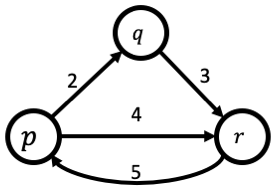
\includegraphics[scale=0.5]{major/order.png}
\end{center}

Your goal is to find an ordering of vertices such that the maximum cost of a node is minimised. In other words, you have to find an ordering such that the cost function $\max_{v \in V}{c(v)}$, is minimised. Design an algorithm for this problem. Give proof of correctness and running time analysis.

\begin{solution}
We claim that the following greedy strategy works:

If the graph is empty, return. Else, find the vertex with the min sum of outgoing edges in the graph, add this vertex to the ordering, and remove this vertex from the graph, and recurse on the
    remaining graph.

Define $V(S)$ to be the value of the cost function of an ordering $S$.

    \textit{Proof:}

    \textbf{Exchange lemma:} For any solution $OS$, there is a solution $OS'$ whose first step coincides with the greedy strategy such that $V(OS) \ge V(OS')$.

    \textit{Proof:}

    Let the vertex $v$ be the vertex chosen in the greedy step.

    Note that apart from $v$, $c(u)$ doesn't increase for any other vertex $u$ in the order.

    We now do a case analysis.

    \begin{enumerate}
    \item The vertex that maximizes $c(u)$ in $OS$ is at the front: $c(u)$ can be at most $c(v)$ by the definition of $v$. Hence by the observation just above this claim, we are done, since $V(OS')
    \le V(OS)$.
    \item The vertex $u$ that maximizes $c(u)$ in $OS$ is not in the front.
        \begin{enumerate}
        \item It is not $v$:
            If it is not $v$, then in $OS'$, $c(u)$ doesn't increase, so we are done in this case.
        \item It is $v$:
            In this case, note that since the first vertex must have cost at least that of $v$ in this ordering, the only possible case is when the first vertex and $v$ have the same cost in the
            ordering, and no outgoing edge from $v$ has an endpoint to the left of v in OS. Hence in this case, we also have $V(OS') \le V(OS)$.
        \end{enumerate}
    \end{enumerate}

Hence we have proved the exchange lemma.

    \textit{Proof by induction:}

    We induct on the number of vertices in $G$.

    If $G$ is empty, we are done.

    Otherwise, consider any solution $OS$, and let $OS'$ be the solution that we build using the exchange lemma. Let $GS$ be the greedy solution, and let $GS'$ and $OS''$ be the order of the remaining
    vertices when the first vertex $v$ is removed from both of them.

    Then we have $V(GS) = \min(c(v), V(GS')) \le \min(c(v), V(OS'')) = V(OS') \le V(OS)$, where the first inequality holds by induction hypothesis.

    Hence we have shown that $V(GS) \le V(OS)$ for all solutions $OS$.

    Specializing to the case where $OS$ is an optimal solution, $V(GS)$ is at most the value of an optimal solution, and hence $GS$ is optimal.


    \textbf{Algorithm:}

    \begin{algorithmic}
        \Function{Q3}{$G = (V, E), w$}
            \State let $q$ := empty min heap
            \State let $c$ := empty array of size $|V|$ filled with $0$s
            \For{$v \in V$}
                \State insert $v$ into $q$ with key $c[v] =$ sum of the weights of outgoing edges from $v$
            \EndFor
            \State let $answer := []$
            \While{$q$ is non empty}
                \State remove the top element of $q$, say $u$
                \State add $u$ to the end of $answer$
                \For{$v$ such that $(u, v) \in E$}:
                    \State decrease key of $v$ from $c[v]$ to $c[v] - w((u, v))$
                \EndFor
            \EndWhile
            \State \Return $answer$
        \EndFunction
    \end{algorithmic}

\textbf{Runtime analysis:}

Creating an empty array takes $O(V)$ time. Creating empty priority queue takes $O(1)$ time. Inserting all vertices takes $O(E + V \log V)$ time where $E$ is for computing c-values and $V \log V$ for
inserting. Removing vertices takes $O(V \log V)$ total time, and decreasing key takes $O(E \log V)$ total time. Adding vertices to $answer$ takes $O(V)$ total time, and returning $answer$ takes
$O(V)$ time.

Hence the time complexity is $O((E + V) \log V)$. Note that this algorithm is like Dijkstra's algorithm, and hence can be solved in a complexity similar to that of an implementation of
Dijkstra's algorithm.
\end{solution}

\question[8]

A teacher wants to use scores $S[1 \dots n]$ (out of $100$) of $n$ students in three subjects (say, physics, chemistry, and mathematics) to locate all the good students in class. The teacher does not
want to use the aggregate score since the subjects are very different in nature and summing the scores does not capture the overall proficiency of a student. Instead, the teacher defines a relation
    ``as-good-as" between pairs of students. Student $i$ is said to be ``as-good-as" another student $j$ iff $S[i].p \geq S[j].p, S[i].c \geq S[j].c, S[i].m \geq S[j].m$ (that is, when student $i$ has
$\geq$ score than student $j$ in all three subjects). Having defined this relation, the teacher now wants to find a list $L$ of all students such that for every student $s \in L$, no other student in
the class is ``as-good-as" $s$. You may assume that no two students have the exact same scores on all three subjects. Design an algorithm for this problem. Give proof of correctness and running time analysis.

[Note that there is a trivial $O(n^2)$ algorithm for this problem. So, you will not receive any points for an $\Omega(n^2)$ algorithm.]

\begin{solution}
    We shall give an algorithm for $d = 2, 3$ dimensions, instead of just 3 (for the sake of completeness). The second of these algorithms is generalizable for $d \ge 4$ as well.

    \textbf{$O(n \log n)$ algorithm for $d = 2$}
    \begin{algorithmic}
        \Function{ParetoOptimalIndices2D}{$S[1 \ldots n]$}
            \State let $a := $ the identity permutation array of size $n$
            \State sort $a$ by the lexicographical order of $S$
            \Function{Helper}{$a[1 \ldots n]$}
                \If{$n = 1$}
                    \State \Return $\{a[1]\}$
                \EndIf
                \State let $b := $ \Call{Helper}{$a[1 \ldots \lfloor n/2 \rfloor]$}
                \State let $c := $ \Call{Helper}{$a[\lfloor n/2 \rfloor + 1 \ldots n]$}
                \State let $y_{max} := \max_{i \in c} S[i].y$
                \State let $b' := \{i \mid i \in b \land S[i].y \ge y_{max}\}$
                \State \Return $b' \cup c$
            \EndFunction
            \State \Return \Call{Helper}{$a$}
        \EndFunction
    \end{algorithmic}

    \textbf{Proof of correctness:}
    We do a brief induction. The base case works clearly. Since all $x$ values of indices in $b$ are lower than those in $c$, and the inductive hypothesis works for $c$, the indices in $c$ must be
    in the answer. Any other index must be in the left part of $a$, and thus in $b$. The only ones which are in the answer must not be dominated by any element of $c$, and hence must have a higher
    $y$ coordinate, which is precisely what we return apart from $c$.

    Note that at this point, it is sufficient to find the subset of $S$ itself, and not the specific indices (they can be found by sorting and doing a linear merge-like step for finding
    the corresponding indices). Hence the following algorithms will merely find the subset and not indices.

    \textbf{Runtime analysis:}
    The first sorting takes $O(n \log n)$ time. If the time taken by a call to \textsc{Helper} is $T(n)$, then we have $T(n) = 2T(n/2) + O(n)$ which means $T(n) = O(n \log n)$. Returning takes $O(n)$
    time, so the overall algorithm takes $O(n \log n)$ time, as claimed.

    \textbf{$O(n \log^2 n)$ algorithm for $d = 3$}
    \begin{algorithmic}
        \Function{ParetoOptimal3D}{$S[1 \ldots n]$}
            \State sort $S$ in lexicographical order
            \Function{Helper}{$S[1 \ldots n]$}
                \If{$n = 1$}
                    \State \Return $S$
                \EndIf
                \State let $A :=$ \Call{Helper}{$S[1 \ldots \lfloor n/2 \rfloor]$}
                \State let $B :=$ \Call{Helper}{$S[\lfloor n/2 \rfloor + 1 \ldots n]$}
                \State let $B' :=$ 2D Pareto-optimal set of $B$ after disregarding the first dimension
                \State sort $B'$ in decreasing order of second coordinate (thus increasing order of third coordinate)
                \State let $A' := []$
                \For{$(x, y, z) \in A$}
                    \State binary search for the least $y'$ in $B'$ satisfying $y' \ge y$
                    \If{no such $y'$ exists}
                        \State add $(x, y, z)$ to $A'$
                    \Else
                        \State let $z'$ be the corresponding $z-$value
                        \If{$z' < z$}
                            \State add $(x, y, z)$ to $A'$
                        \EndIf
                    \EndIf
                \EndFor
                \State \Return $A' \cup B$
            \EndFunction
            \State \Return \Call{Helper}{$S$}
        \EndFunction
    \end{algorithmic}

    \textbf{Proof of correctness:}

    We induct on $n$, and assume that the inputs to \textsc{Helper} are always sorted in lexicographical order, which is what the first line ensures.

    Note that in the base case, we are done.

    Now note that all points in $B$ dominate points in $A$, and no two of them dominate each other. Hence this set must be in the answer. The points not in $B$ must come from $S[1 \ldots
    \lfloor n/2 \rfloor]$, and since they must not dominate each other, they must form a subset of $A$. The points in the answer must not be dominated by points in $B$, and hence there must be no
    point in $B$ which dominates it in both the $y$ and the $z$ coordinates. Note that if we sort a 2D pareto optimal set in the increasing order of $x-$coordinate (duplicate $x-$coordinates
    would lead to a contradiction to the definition of Pareto-optimality), then it is sorted in the decreasing order of $y-$coordinate. Hence, if there exists a $(y', z')$ that dominates $(y, z)$,
    then any point $(y'', z'')$ in the Pareto-optimal set $B'$ which satisfies $y' \ge y'' \ge y$ dominates $(y, z)$ as well. Hence we can find the least such $y'$ and be done with the decision to
    include/exclude $(x, y, z)$ in the final answer or not.
    Since we argued that the answer will be a subset of the subset so found (by necessity arguments), we merely have to note that the formed subset is indeed Pareto-optimal, which is easy to
    see. Hence our proof by induction is complete, and we are done.

    \textbf{Runtime analysis:}

    Note that the initial sorting takes $O(n \log n)$ time. Suppose the call to \textsc{Helper} takes $T(n)$ time. Then $T(1) = 1$. When $n > 1$, the time taken by recursive calls is
    roughly $2T(n / 2)$, and sorting and binary searching for all elements takes $O(n \log n)$ time. Hence we have $T(n) = 2T(n / 2) + O(n \log n)$, which gives us $T(n) = O(n \log^2 n)$.
    Returning the answer takes $O(n)$ time as well, and hence the final complexity of the algorithm is $O(n \log^2 n)$.

    Now we shall give an algorithm that unrolls the recursion and avoids the recomputation of the 2D Pareto-optimal set to ensure that the complexity is $O(n \log n)$.

    \textbf{$O(n \log n)$ algorithm for $d = 3$}
    \begin{algorithmic}
        \Function{ParetoOptimal3D}{$S[1 \ldots n]$}
            \State sort $S$ in reverse lexicographical order
            \State let $T := $ an empty ordered/indexed set of 2-tuples, ordered in reverse lexicographical order*
            \State \Comment{Invariant: after the $i^\mathrm{th}$ iteration, $T$ is sorted in increasing order of $z$ and decreasing order of $y$, and is the Pareto-optimal set of $\{(y, z) \mid (x, y, z) \in S[1\ldots i]\}$}
            \State $answer := \{\}$
            \For{$i \in \{1, \ldots, n\}$}
                \State find the leftmost element in $T$ whose $y$-coordinate is $\ge S[i].y$
                \If{such an element exists and the corresponding $z$-coordinate is $\ge S[i].z$}
                    \State continue
                \EndIf
                \State add $S[i]$ to $answer$
                \State binary search for the leftmost element which has $y \le S[i].y$.
                \State binary search for the rightmost element which has $z \le S[i].z$.
                \State remove all elements between these elements (both inclusive) (if this range is non-empty) from $T$ and insert $(S[i].y, S[i].z)$ into $T$.
            \EndFor
            \State \Return $answer$
        \EndFunction
    \end{algorithmic}

    *For instance, GNU C++'s policy based data structure order statistics red-black tree, or a hand-written AVL tree capable of binary search on both coordinates (given the invariant) and iterating over a range $[i, j]$ of indices in
    $O((j-i+1)\log n)$ time.

    \textbf{Proof of correctness:}

    \textbf{Claim 1:} If $S[i]$ is dominated by $S[j]$ and $i \ne j$, then $i > j$.

    \textit{Proof:} Suppose $i < j$. Then since $S[i]$ comes before $S[j]$, either $S[i].x > S[j].x$, or $S[i].x = S[j].x \land S[i].y > S[j].y$, or $S[i].x = S[j].x \land S[i].y = S[j].y \land
    S[i].z > S[j].z$. Note that $S[i] \ne S[j]$ since all elements are distinct (if they aren't, preprocessing can get rid of them in $O(n \log n)$). In any case, $S[i]$ is not dominated by $S[j]$,
    which is a contradiction.

    \textbf{Claim 2:} The invariant is satisfied after each iteration.
    
    \textit{Proof:} We perform an induction on the iteration number in the loop.

    Base case: The invariant is true after the 0th iteration.
    
    Inductive step: Firstly, if there is an element in $T$ that dominates $(S[i].y, S[i].z)$, then by the inductive hypothesis, the leftmost element of $T$ with $y \ge S[i].y$ must also
    dominate $T$. If such an element dominates, we do nothing to $T$ (since the new element can't be part of $T$), and the invariant holds in this case.

    Now consider any element $(y, z)$ in $T$ which is dominated by $(S[i].y, S[i].z)$ (if any such element exists at all). Since $T$ is sorted in decreasing order by $y$ and increasing order by $z$,
    $(y, z)$ must come at or after the leftmost element with $y \le S[i].y$, and at or before the element with $z \le S[i].z$. Hence if we replace all these elements by $(S[i].y, S[i].z)$, then the ordering of $y$ and $z$ remains the same as before, owing to the definition of which
    range was replaced. Also, all elements that are dominated by $(S[i].y, S[i].z)$ are replaced (and only those elements are replaced).
    Hence our inductive step is complete, and so is our proof.

    \textbf{Claim 3:} $S[i]$ is in the Pareto-optimal set of $S$ iff for any $(y, z) \in T, (S[i].y, S[i].z)$ is not dominated by $(y, z)$ (here $T$ is the copy before the $i^\mathrm{th}$
    iteration).
    
    \textit{Proof:} Note that $S[i]$ can't be dominated by any $S[j]$ with $j > i$. For all $j < i$, we have $S[j].x \ge S[i].x$, hence if there exists any $S[j]$ with $j < i$ whose $(y, z)$ dominate
    those of $S[i]$, then $S[i]$ must not be in the answer. However, if there is no such $S[j]$, then since $S[i]$ isn't dominated by anything on the right as well as the left, it must be in the
    answer. Note that this translates to checking if $(S[i].y, S[i].z)$ is dominated by $(y, z)$ of any of its predecessors, and since $T$ maintains the Pareto-optimal set of these pairs, it is
    equivalent to checking if there is a $(y, z)$ in $T$ which dominates $(S[i].y, S[i].z)$ or not.

    \textbf{Runtime analysis:}
    Sorting takes $O(n \log n)$ time.
    Note that insertion and deletion takes $O(\log n)$ time from such a tree, and since there are at most $n$ insertions and deletions, the time taken is $O(n \log n)$ for construction of $T$, and
    the contruction and returning of $answer$ takes $O(n)$ time, and hence the overall time complexity is $O(n \log n)$.

\end{solution}

\question[8]

You are the technical manager at a match-making service and your task for the day is to perfectly match $X = \{x_1, ...., x_n\}$ with $Y = \{y_1, ..., y_n\}$. You are given a weighted edge set $E$
consisting of edges between one node of $X$ and one node in $Y$. So, $(X, Y, E)$ form a bipartite graph. There is a positive weight $c((x, y)) > 0$ associated with every edge $(x, y) \in E$ that
denotes the compatibility of the pair $x-y$. The quality of a matching is equal to the minimum compatibility edge in that matching (in some sense, the worst pair in the matching determines the quality of the matching).

For example, consider the bipartite graph given below on the left. The quality of the matching (shown in red) in the middle figure is $1$ whereas the quality of the matching in the right figure is
$2$.

\begin{center}
    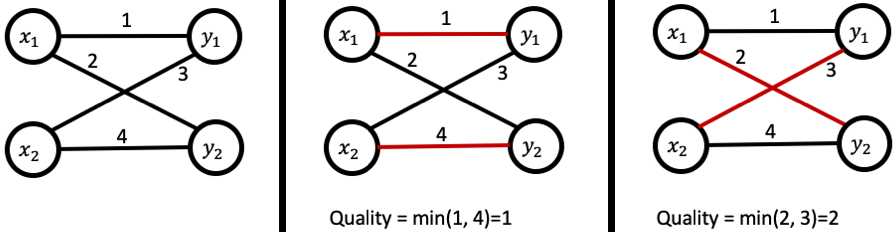
\includegraphics[scale=0.4]{major/Match.png}
\end{center}

Your goal is to find a perfect matching such that the quality of the matching is maximised. You may assume that there exists a perfect matching. Design an algorithm for this problem. Give proof of correctness and running time analysis.

[There are points for efficiency.]
\begin{solution}

    Let $n = |V|, m = |E|$. We first come up with a solution that uses binary search, and then remove the extra $\log n$ factor by running a modified form of the Ford-Fulkerson algorithm.

    \textbf{Algorithm:}

    \begin{algorithmic}
        \Function{Matching}{$G = (X, Y, E)$}
            \State sort $E$ by weights
            \State $l := 1$
            \State $r := |E|$
            \State $minWeightEdge := 1$
            \While{$l \le r$}
                \State $m := \lfloor (l + r) / 2 \rfloor$
                \State $E' := E \setminus \{e \mid w(e) < w(E[m])\}$
                \If{there is a perfect matching in $(X, Y, E)$}
                    \State $minWeightEdge := m$
                    \State $l := m + 1$
                \Else
                    \State $r := m - 1$
                \EndIf
            \EndWhile
            \State \Return perfect matching in $(X, Y, E \setminus \{e \mid w(e) < w(E[minWeightEdge])\})$
        \EndFunction
    \end{algorithmic}

    \textbf{Proof of correctness:}

    Let $P(e)$ be the problem where we need to output whether there is a perfect matching in the graph whose min-weight edge has cost at least $e$, and let $S(e)$ be the answer to the problem.

    Note that the problem reduces to finding the maximum $e$ such that $S(e)$ is true.

    \textbf{Claim 1:} If $S(e)$ is true, then $S(f)$ is true for all $f < e$.

    \textit{Proof:} Consider the perfect matching corresponding to $P(e)$ in this case. Since the min-weight edge has weight at least $e$, and $e > f$, the min-weight edge has weight at least $f$.
    Hence the answer to $P(f)$ is true as well, as we have shown the existence of such a perfect matching.

    \textbf{Claim 2:} At any iteration in the while loop, either $[l, r]$ has at least one edge with cost $e$ with $P(e)$ true, or $minWeightEdge$ corresponds to the edge with the maximum $e$ such
    that $S(e)$ is true and $r < minWeightEdge$. We also have that $S(minWeightEdge)$ is always true.

    \textit{Proof:} Before the first iteration, this is true, since there must be at least one edge (since the perfect matching is guaranteed to exist), and the weight of the edge with index 1 in the
    sorted order satisfied $S(e)$ = true (since weight of an edge in the graph is at least the min weight of an edge). Now suppose at a certain iteration, we are at $l, r$. Then if the answer is in
    $[l, r]$, we check the middle edge. If it works, then the answer must be in $[l, m]$, and we store $m$ in $minWeightEdge$, and we need to search $[l, m - 1]$. Else if it is not, then the answer is
    in $[m+1, r]$ or stored already in $minWeightEdge$. If in the previous iteration, the answer does not exist in $[l, r]$, $minWeightEdge$ already stores it and $[m+1, r]$ has $r <
    minWeightEdge$, and if the answer exists in $[l, r]$, then the answer is not in $[l, m - 1]$ because of Claim 1, so it must exist in $[m + 1, r]$ or $minWeightEdge$ already stores it. Hence we have shown that Claim 2 is true.

    From Claim 2, applying it to the last iteration (after which we have $l > r$), we see that the algorithm answers the problem correctly.

    \textbf{Runtime analysis:}
    Sorting takes $O(m \log m)$ time. Whenever we check for a perfect matching, it takes $O(n(n + m))$ time since the max matching can be at most $n$. At every step, the value of $r - l$ decreases by at least half, and hence the
    number of iterations is $O(\log m)$ since $r - l$ is initially $m - 1$. Hence the total time in the binary search takes $O(n(n + m) \log m)$ time. Returning the final perfect matching takes
    $O(n(n + m))$ time
    as well, so the overall time complexity is $O(n(n + m) \log m) = O(n(n + m) \log n)$, since $m \in O(n^2)$.
\end{solution}

\begin{solution}

    Now we shall exhibit a better algorithm:

    \begin{algorithmic}
        \Function{Matching}{$G = (X, Y, E)$}
            \State sort $E$ in the non-increasing order of weights
            \State let $H$ be a graph with source vertex $s$, sink vertex $t$, all $x_i$ connected to $s$ with a directed edge from $s$, all $y_i$ connected to $t$ with a directed edge from $y_i$,
            all edges with capacity 1.
            \State let $H'$ be the reverse graph of $H$.
            \State let $visited_s := $ boolean array of size $2n$ initialized with the first half false and second half true
            \State let $visited_t := $ boolean array of size $2n$ initialized with the second half false and first half true
            \State let $matchingSize := 0$
            \State let $i := 1$
            \While{$i \le n$}
                \State let $(x_a, y_b) := E[i]$
                \State add $(x_a, y_b)$ to $H$ and $(y_b, x_a)$ to $H'$ with capacity 1 and flow value 0
                \State $i := i + 1$
                \If{$(visited_s[x] \land visited_t[y]) \lor (visited_t[x] \land visited_s[y])$}
                    \State run Ford Fulkerson on the residual graphs of $H$ and $H'$ computed so far
                    \State using dfs on the residual graph of $H$, recompute $visited_s$
                    \State using dfs on the residual graph of $H'$, recompute $visited_t$
                    \State $matchingSize := $ value of the flow so found
                    \If{$matchingSize = n$}
                        \State \Return the corresponding matching found
                    \EndIf
                \Else
                    \State recompute $visited_s, visited_t$ using dfs on the residual graphs of $H, H'$
                \EndIf
            \EndWhile
        \EndFunction
    \end{algorithmic}

    \textbf{Proof of correctness:}

    \textbf{Claim 1:} After the $i^\mathrm{th}$ iteration, the following statements are true:
        \begin{enumerate}
            \item $H$ is the graph formed after adding $E[1\ldots i]$, and $H'$ is the reverse of $H$.
            \item $visited_s[v]$ is true iff $x_v$ can be visited from $s$ by a path in the residual graph of $H$.
            \item $visited_t[v]$ is true iff $t$ can be visited from $y_v$ by a path in the residual graph of $H$.
            \item $visited_s$ and $visited_t$ are disjoint.
            \item $matchingSize$ equals the max flow in the graph $H$ (which is the size of the maximum matching in the graph).
        \end{enumerate}
    
    \textit{Proof:} We proceed with induction.

    Base case: This is true for $i = 0$ since only $x_i$'s can be visited from $t$, and $t$ can be visited only from $y_i$'s, and there is 0 flow in the network.

    Induction step: Suppose this is true for some $i^\mathrm{th}$ iteration. In the next iteration, we add $E[i]$ to both $H$ and $H'$ in different orientations. If both $x, y$ can be visited from $s$, then there is no flow augmentation possible, since $t$ is
    not reachable from any of them, as $visited_s, visited_t$ are disjoint. Similarly, if $t$ can be visited from $x, y$, then neither of $x, y$ can be visited from $s$, so there is no flow
    augmentation possible. If one of the vertices is unreachable from $s$ or can't reach $t$, then there is no flow augmentation possible either. Hence the only remaining case is when one of them can be visited from $s$ and $t$ can be visited from the other one. In this case, we can augment the path, and the flow
    increases by at least $1$, since the capacity of this edge is $1$ and there is no flow through it. Running Ford Fulkerson ensures that there is no remaining augmenting path, and hence the
    vertices that can be visited from $s$ have no path to $t$. Similarly, vertices that have a path to $t$ can't be visited from $s$ (by the contrapositive or considering $H'$), and are hence
    disjoint.
    In all the cases where flow augmentation is possible (which are precisely those cases where the flow can increase), we update $matchingSize$ as well. Also, wherever there is no flow augmentation,
    we update $visited_s, visited_t$ just to maintain the invariant.
    Hence this completes the inductive step and we are done.

    Now that this claim is proven, we can note that this algorithm does a linear search on $S(e)$ as defined in the previous solution in the decreasing order of edge weights, stopping if it finds the
    answer, and hence should give the correct answer.

    \textbf{Runtime analysis:}

    Creation of the graphs takes $O(n + m)$ time, and sorting the edges takes $O(m \log m)$ time. Now note that running Ford Fulkerson on a partial residual graph takes $O(a \times (n + m)$ time,
    where $a$ is the number of iterations. Whenever we run Ford Fulkerson, we also recompute $visited_s, visited_t$ and compute the flow value as well. This takes $O(n + m)$ time as well. So
    whenever we run Ford Fulkerson, the time taken is $O((a + 1)(n + m))$, and otherwise we just do $O(n + m)$ work. Hence the total work done in the loop is $O(n (n + m) + \sum(a + 1)(n + m))$ where the sum is taken over
    all possible runs of Ford Fulkerson. Note that whenever we run Ford Fulkerson, we are guaranteed to get at least an increase of 1 in the flow value. Hence there can be at most $n$ total
    iterations of Ford Fulkerson (since maximum matching can't exceed $n$). Thus, the sum of $a$ is at most $n$, and the number of summands is also at most $n$. So the total work done in the loop is
    $O(n (n + m))$. Returning the found matching takes $O(n + m)$ time as well. So the overall runtime is $O(n(n + m) + m \log m) = O(m(n + \log m) + n^2) = O(m(n + n) + n^2) = O(n(n + m))$,
    where $\log m \in o(n)$ since $m \in O(n^2)$.

\end{solution}

\end{questions}
\end{document}

